
%% bare_conf.tex
%% V1.4b
%% 2015/08/26
%% by Michael Shell
%% See:
%% http://www.michaelshell.org/
%% for current contact information.
%%
%% This is a skeleton file demonstrating the use of IEEEtran.cls
%% (requires IEEEtran.cls version 1.8b or later) with an IEEE
%% conference paper.
%%
%% Support sites:
%% http://www.michaelshell.org/tex/ieeetran/
%% http://www.ctan.org/pkg/ieeetran
%% and
%% http://www.ieee.org/

%%*************************************************************************
%% Legal Notice:
%% This code is offered as-is without any warranty either expressed or
%% implied; without even the implied warranty of MERCHANTABILITY or
%% FITNESS FOR A PARTICULAR PURPOSE! 
%% User assumes all risk.
%% In no event shall the IEEE or any contributor to this code be liable for
%% any damages or losses, including, but not limited to, incidental,
%% consequential, or any other damages, resulting from the use or misuse
%% of any information contained here.
%%
%% All comments are the opinions of their respective authors and are not
%% necessarily endorsed by the IEEE.
%%
%% This work is distributed under the LaTeX Project Public License (LPPL)
%% ( http://www.latex-project.org/ ) version 1.3, and may be freely used,
%% distributed and modified. A copy of the LPPL, version 1.3, is included
%% in the base LaTeX documentation of all distributions of LaTeX released
%% 2003/12/01 or later.
%% Retain all contribution notices and credits.
%% ** Modified files should be clearly indicated as such, including  **
%% ** renaming them and changing author support contact information. **
%%*************************************************************************


% *** Authors should verify (and, if needed, correct) their LaTeX system  ***
% *** with the testflow diagnostic prior to trusting their LaTeX platform ***
% *** with production work. The IEEE's font choices and paper sizes can   ***
% *** trigger bugs that do not appear when using other class files.       ***                          ***
% The testflow support page is at:
% http://www.michaelshell.org/tex/testflow/



\documentclass[conference]{IEEEtran}
% Some Computer Society conferences also require the compsoc mode option,
% but others use the standard conference format.
%
% If IEEEtran.cls has not been installed into the LaTeX system files,
% manually specify the path to it like:
% \documentclass[conference]{../sty/IEEEtran}





% Some very useful LaTeX packages include:
% (uncomment the ones you want to load)


% *** MISC UTILITY PACKAGES ***
%
%\usepackage{ifpdf}
% Heiko Oberdiek's ifpdf.sty is very useful if you need conditional
% compilation based on whether the output is pdf or dvi.
% usage:
% \ifpdf
%   % pdf code
% \else
%   % dvi code
% \fi
% The latest version of ifpdf.sty can be obtained from:
% http://www.ctan.org/pkg/ifpdf
% Also, note that IEEEtran.cls V1.7 and later provides a builtin
% \ifCLASSINFOpdf conditional that works the same way.
% When switching from latex to pdflatex and vice-versa, the compiler may
% have to be run twice to clear warning/error messages.






% *** CITATION PACKAGES ***
%
%\usepackage{cite}
% cite.sty was written by Donald Arseneau
% V1.6 and later of IEEEtran pre-defines the format of the cite.sty package
% \cite{} output to follow that of the IEEE. Loading the cite package will
% result in citation numbers being automatically sorted and properly
% "compressed/ranged". e.g., [1], [9], [2], [7], [5], [6] without using
% cite.sty will become [1], [2], [5]--[7], [9] using cite.sty. cite.sty's
% \cite will automatically add leading space, if needed. Use cite.sty's
% noadjust option (cite.sty V3.8 and later) if you want to turn this off
% such as if a citation ever needs to be enclosed in parenthesis.
% cite.sty is already installed on most LaTeX systems. Be sure and use
% version 5.0 (2009-03-20) and later if using hyperref.sty.
% The latest version can be obtained at:
% http://www.ctan.org/pkg/cite
% The documentation is contained in the cite.sty file itself.






% *** GRAPHICS RELATED PACKAGES ***
%
\ifCLASSINFOpdf
  % \usepackage[pdftex]{graphicx}
  % declare the path(s) where your graphic files are
  % \graphicspath{{../pdf/}{../jpeg/}}
  % and their extensions so you won't have to specify these with
  % every instance of \includegraphics
  % \DeclareGraphicsExtensions{.pdf,.jpeg,.png}
\else
  % or other class option (dvipsone, dvipdf, if not using dvips). graphicx
  % will default to the driver specified in the system graphics.cfg if no
  % driver is specified.
  % \usepackage[dvips]{graphicx}
  % declare the path(s) where your graphic files are
  % \graphicspath{{../eps/}}
  % and their extensions so you won't have to specify these with
  % every instance of \includegraphics
  % \DeclareGraphicsExtensions{.eps}
\fi
% graphicx was written by David Carlisle and Sebastian Rahtz. It is
% required if you want graphics, photos, etc. graphicx.sty is already
% installed on most LaTeX systems. The latest version and documentation
% can be obtained at: 
% http://www.ctan.org/pkg/graphicx
% Another good source of documentation is "Using Imported Graphics in
% LaTeX2e" by Keith Reckdahl which can be found at:
% http://www.ctan.org/pkg/epslatex
%
% latex, and pdflatex in dvi mode, support graphics in encapsulated
% postscript (.eps) format. pdflatex in pdf mode supports graphics
% in .pdf, .jpeg, .png and .mps (metapost) formats. Users should ensure
% that all non-photo figures use a vector format (.eps, .pdf, .mps) and
% not a bitmapped formats (.jpeg, .png). The IEEE frowns on bitmapped formats
% which can result in "jaggedy"/blurry rendering of lines and letters as
% well as large increases in file sizes.
%
% You can find documentation about the pdfTeX application at:
% http://www.tug.org/applications/pdftex





% *** MATH PACKAGES ***
%
%\usepackage{amsmath}
% A popular package from the American Mathematical Society that provides
% many useful and powerful commands for dealing with mathematics.
%
% Note that the amsmath package sets \interdisplaylinepenalty to 10000
% thus preventing page breaks from occurring within multiline equations. Use:
%\interdisplaylinepenalty=2500
% after loading amsmath to restore such page breaks as IEEEtran.cls normally
% does. amsmath.sty is already installed on most LaTeX systems. The latest
% version and documentation can be obtained at:
% http://www.ctan.org/pkg/amsmath





% *** SPECIALIZED LIST PACKAGES ***
%
%\usepackage{algorithmic}
% algorithmic.sty was written by Peter Williams and Rogerio Brito.
% This package provides an algorithmic environment fo describing algorithms.
% You can use the algorithmic environment in-text or within a figure
% environment to provide for a floating algorithm. Do NOT use the algorithm
% floating environment provided by algorithm.sty (by the same authors) or
% algorithm2e.sty (by Christophe Fiorio) as the IEEE does not use dedicated
% algorithm float types and packages that provide these will not provide
% correct IEEE style captions. The latest version and documentation of
% algorithmic.sty can be obtained at:
% http://www.ctan.org/pkg/algorithms
% Also of interest may be the (relatively newer and more customizable)
% algorithmicx.sty package by Szasz Janos:
% http://www.ctan.org/pkg/algorithmicx




% *** ALIGNMENT PACKAGES ***
%
%\usepackage{array}
% Frank Mittelbach's and David Carlisle's array.sty patches and improves
% the standard LaTeX2e array and tabular environments to provide better
% appearance and additional user controls. As the default LaTeX2e table
% generation code is lacking to the point of almost being broken with
% respect to the quality of the end results, all users are strongly
% advised to use an enhanced (at the very least that provided by array.sty)
% set of table tools. array.sty is already installed on most systems. The
% latest version and documentation can be obtained at:
% http://www.ctan.org/pkg/array


% IEEEtran contains the IEEEeqnarray family of commands that can be used to
% generate multiline equations as well as matrices, tables, etc., of high
% quality.




% *** SUBFIGURE PACKAGES ***
%\ifCLASSOPTIONcompsoc
%  \usepackage[caption=false,font=normalsize,labelfont=sf,textfont=sf]{subfig}
%\else
%  \usepackage[caption=false,font=footnotesize]{subfig}
%\fi
% subfig.sty, written by Steven Douglas Cochran, is the modern replacement
% for subfigure.sty, the latter of which is no longer maintained and is
% incompatible with some LaTeX packages including fixltx2e. However,
% subfig.sty requires and automatically loads Axel Sommerfeldt's caption.sty
% which will override IEEEtran.cls' handling of captions and this will result
% in non-IEEE style figure/table captions. To prevent this problem, be sure
% and invoke subfig.sty's "caption=false" package option (available since
% subfig.sty version 1.3, 2005/06/28) as this is will preserve IEEEtran.cls
% handling of captions.
% Note that the Computer Society format requires a larger sans serif font
% than the serif footnote size font used in traditional IEEE formatting
% and thus the need to invoke different subfig.sty package options depending
% on whether compsoc mode has been enabled.
%
% The latest version and documentation of subfig.sty can be obtained at:
% http://www.ctan.org/pkg/subfig




% *** FLOAT PACKAGES ***
%
%\usepackage{fixltx2e}
% fixltx2e, the successor to the earlier fix2col.sty, was written by
% Frank Mittelbach and David Carlisle. This package corrects a few problems
% in the LaTeX2e kernel, the most notable of which is that in current
% LaTeX2e releases, the ordering of single and double column floats is not
% guaranteed to be preserved. Thus, an unpatched LaTeX2e can allow a
% single column figure to be placed prior to an earlier double column
% figure.
% Be aware that LaTeX2e kernels dated 2015 and later have fixltx2e.sty's
% corrections already built into the system in which case a warning will
% be issued if an attempt is made to load fixltx2e.sty as it is no longer
% needed.
% The latest version and documentation can be found at:
% http://www.ctan.org/pkg/fixltx2e


%\usepackage{stfloats}
% stfloats.sty was written by Sigitas Tolusis. This package gives LaTeX2e
% the ability to do double column floats at the bottom of the page as well
% as the top. (e.g., "\begin{figure*}[!b]" is not normally possible in
% LaTeX2e). It also provides a command:
%\fnbelowfloat
% to enable the placement of footnotes below bottom floats (the standard
% LaTeX2e kernel puts them above bottom floats). This is an invasive package
% which rewrites many portions of the LaTeX2e float routines. It may not work
% with other packages that modify the LaTeX2e float routines. The latest
% version and documentation can be obtained at:
% http://www.ctan.org/pkg/stfloats
% Do not use the stfloats baselinefloat ability as the IEEE does not allow
% \baselineskip to stretch. Authors submitting work to the IEEE should note
% that the IEEE rarely uses double column equations and that authors should try
% to avoid such use. Do not be tempted to use the cuted.sty or midfloat.sty
% packages (also by Sigitas Tolusis) as the IEEE does not format its papers in
% such ways.
% Do not attempt to use stfloats with fixltx2e as they are incompatible.
% Instead, use Morten Hogholm'a dblfloatfix which combines the features
% of both fixltx2e and stfloats:
%
% \usepackage{dblfloatfix}
% The latest version can be found at:
% http://www.ctan.org/pkg/dblfloatfix




% *** PDF, URL AND HYPERLINK PACKAGES ***
%
%\usepackage{url}
% url.sty was written by Donald Arseneau. It provides better support for
% handling and breaking URLs. url.sty is already installed on most LaTeX
% systems. The latest version and documentation can be obtained at:
% http://www.ctan.org/pkg/url
% Basically, \url{my_url_here}.




% *** Do not adjust lengths that control margins, column widths, etc. ***
% *** Do not use packages that alter fonts (such as pslatex).         ***
% There should be no need to do such things with IEEEtran.cls V1.6 and later.
% (Unless specifically asked to do so by the journal or conference you plan
% to submit to, of course. )


\usepackage{graphicx}


% correct bad hyphenation here
\hyphenation{op-tical net-works semi-conduc-tor}


\usepackage{syntax}
\grammarindent 80pt

\usepackage{newfloat}
% declare the floating environment {Grammar}
% this will also define \listofGrammars:
\DeclareFloatingEnvironment[
% the file extension for the file used to create the list:
fileext   = logr,% don't use log here!
% the heading for the list:
listname  = {List of Grammars},
% the name used in captions:
name      = Gramática,
% the default floating parameters if the environment is used
% without optional argument:
placement = htp
]{Grammar}



\begin{document}
%
% paper title
% Titles are generally capitalized except for words such as a, an, and, as,
% at, but, by, for, in, nor, of, on, or, the, to and up, which are usually
% not capitalized unless they are the first or last word of the title.
% Linebreaks \\ can be used within to get better formatting as desired.
% Do not put math or special symbols in the title.
\title{Bare Demo of IEEEtran.cls\\ for IEEE Conferences}


% author names and affiliations
% use a multiple column layout for up to three different
% affiliations
\author{\IEEEauthorblockN{Michael Shell}
\IEEEauthorblockA{School of Electrical and\\Computer Engineering\\
Georgia Institute of Technology\\
Atlanta, Georgia 30332--0250\\
Email: http://www.michaelshell.org/contact.html}
\and
\IEEEauthorblockN{Homer Simpson}
\IEEEauthorblockA{Twentieth Century Fox\\
Springfield, USA\\
Email: homer@thesimpsons.com}
\and
\IEEEauthorblockN{James Kirk\\ and Montgomery Scott}
\IEEEauthorblockA{Starfleet Academy\\
San Francisco, California 96678--2391\\
Telephone: (800) 555--1212\\
Fax: (888) 555--1212}}

% conference papers do not typically use \thanks and this command
% is locked out in conference mode. If really needed, such as for
% the acknowledgment of grants, issue a \IEEEoverridecommandlockouts
% after \documentclass

% for over three affiliations, or if they all won't fit within the width
% of the page, use this alternative format:
% 
%\author{\IEEEauthorblockN{Michael Shell\IEEEauthorrefmark{1},
%Homer Simpson\IEEEauthorrefmark{2},
%James Kirk\IEEEauthorrefmark{3}, 
%Montgomery Scott\IEEEauthorrefmark{3} and
%Eldon Tyrell\IEEEauthorrefmark{4}}
%\IEEEauthorblockA{\IEEEauthorrefmark{1}School of Electrical and Computer Engineering\\
%Georgia Institute of Technology,
%Atlanta, Georgia 30332--0250\\ Email: see http://www.michaelshell.org/contact.html}
%\IEEEauthorblockA{\IEEEauthorrefmark{2}Twentieth Century Fox, Springfield, USA\\
%Email: homer@thesimpsons.com}
%\IEEEauthorblockA{\IEEEauthorrefmark{3}Starfleet Academy, San Francisco, California 96678-2391\\
%Telephone: (800) 555--1212, Fax: (888) 555--1212}
%\IEEEauthorblockA{\IEEEauthorrefmark{4}Tyrell Inc., 123 Replicant Street, Los Angeles, California 90210--4321}}




% use for special paper notices
%\IEEEspecialpapernotice{(Invited Paper)}




% make the title area
\maketitle

% As a general rule, do not put math, special symbols or citations
% in the abstract
\begin{abstract}
The abstract goes here.
\end{abstract}

% no keywords




% For peer review papers, you can put extra information on the cover
% page as needed:
% \ifCLASSOPTIONpeerreview
% \begin{center} \bfseries EDICS Category: 3-BBND \end{center}
% \fi
%
% For peerreview papers, this IEEEtran command inserts a page break and
% creates the second title. It will be ignored for other modes.
\IEEEpeerreviewmaketitle



\section{Introduction}
% no \IEEEPARstart
This demo file is intended to serve as a ``starter file''
for IEEE conference papers produced under \LaTeX\ using
IEEEtran.cls version 1.8b and later.
% You must have at least 2 lines in the paragraph with the drop letter
% (should never be an issue)
I wish you the best of success.

\hfill mds
 
\hfill August 26, 2015

\section{Protein Structure Prediction} \label{sec:proteinfolding}


Proteins are macromolecules composed by an alphabet of twenty different amino acids, also referred to as residues. An amino acid is formed by a peptide backbone and a distinctive side chain group. The peptide bond is defined by an amino group and a carboxyl group connected to an alpha carbon to which a hydrogen and side chain group are attached.


Sequences are formed by combining amino acids and are considered the primary structure of
proteins.
%Amino acids are combined to form sequences which are considered the primary structure of the peptides or proteins. 
The secondary structure is the locally ordered structure brought via hydrogen bounding mainly within the peptide backbone. The most common secondary structure elements in proteins are the alpha helix and the beta sheet. The global folding of a polypeptide chain
is also called as the tertiary structure.

%The tertiary structure is the global folding of a single polypeptide chain.

Under specific conditions, the protein sequence folds into a unique native 3-D structure. Each possible protein fold has an associated energy. The \emph{thermodynamic hypothesis} states that the native structure of a protein is the one for which the free energy achieves the global minimum. Based on this hypothesis, many methods \cite{custodio2004investigation, hsu2003growth, krasnogor2002multimeme, lin2011protein, unger1993genetic} that search for the protein native structure define an approximation of the protein energy and use optimization algorithms that look for the protein fold that minimizes this energy. These approaches mainly differ in the type of energy approximation employed and in the characteristics of the protein modeling.


\subsection{The HP Model} \label{sec:hpModel}


%Using a representation close to the real would be impossible for current computers to process the information in a reasonable time.
The protein structures are very complex. Detailed representation of proteins exist and can be used to model the protein folding, these representations are computationally very costly. Having this in mind, Lau and Dill \cite{lau1989lattice} created a model called \textit{Hydrophobic-Hydrophilic} Model (HP Model), to represent the proteins using simplifications. The model can be used either to represent proteins in a 2D space or 3D space.


The HP model considers two types of residues:  hydrophobic (H) residues  and hydrophilic or polar (P) residues. A protein is considered a sequence of these two types of residues, which are located in regular lattice models forming self-avoided paths. Given a pair of residues, they are considered neighbors if they are adjacent  either in the chain (connected neighbors) or  in the lattice but not connected in the chain (topological neighbors).


\begin{figure}[htb!] \label{fig:PROTEXAM}
	\centering
	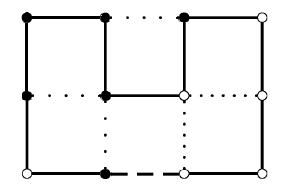
\includegraphics[scale=0.7]{figures/proteinExample.png}
	\caption{One possible configuration of  sequence $PPPPHPHHHHPH$ in the HP model. There is one $HH$ (represented by a dotted line with wide spaces), one $HP$ (represented by a dashed line) and  two $PP$  (represented by dotted lines) contacts.}
\end{figure}


The total number of topological neighboring positions in the lattice ($z$) is called the lattice coordination number.


For the HP model, an energy function that  measures the interaction between topological  neighbor residues is defined  as  $\epsilon_{HH}=-1$ and $\epsilon_{HP}=\epsilon_{PP}=0$. The HP problem consists of finding the solution that minimizes the total energy. In the linear representation of the sequence, hydrophobic residues are represented with the letter H and polar ones, with P. In the graphical representation, hydrophobic proteins are represented  by black beads and polar proteins, by white beads. Figure~\ref{fig:PROTEXAM} shows the graphical representation of a possible configuration for  the sequence  $HHHPHPPPPPH$ in a 2D space. The energy that the HP model associates with this configuration is $-2$ because there is only two $HH$ contact, arisen between the second and fifth residues.


Among many works related to the Protein Folding Problem, here are some examples of the approaches that have been used to solve it.

A very influential paper from Unger and Moult  \cite{unger1993genetic}, introduces a evolutionary algorithm (EA) which uses heuristic-based crossover and mutation operators for the HP model. The algorithm outperformed many variants of Monte Carlo methods for different instances. However,
good results were obtained, the EA was unable to find the global optimal for the longest instances considered.

%
%Alternative
%Unger and Moult \cite{unger1993genetic} described a genetic algorithm (GA) that uses heuristic-based operators for crossover and mutation for the HP model.



A multimeme algorithm (MMA) presented in \cite{krasnogor2002multimeme} is a EA combined with a
group of local search methods. For each individual in the population the MMA, selects a local search method that best fits. Used first to find solutions for the functional model protein. The strategy was later improved with fuzzy-logic-based local searches, leading the algorithm to achieve improved results in the PSP problem.

%The multimeme algorithm (MMA) proposed by \cite{krasnogor2002multimeme} is a GA combined with a set of local search methods. The algorithm, for each different instance or individual in the population, selects the local search method that best fits. 




%Originally used to find solutions for the functional model protein. The algorithm was later improved with fuzzy-logic-based local searches, leading the algorithm to produce improved results in the PSP problem.


In \cite{hsu2003growth}, the author uses  pruned-enriched Rosenbluth method (PERM) also know as Chain growth algorithm, that is based on growing the sequence conformation by adding particle by particle, aiming to increase good configurations and eliminating bad ones.


The ant colony optimization (ACO) was applied to the PSP problem using the HP-2D model in \cite{shmygelska2002ant, shmygelska2003improved}. This strategy, uses artificial ants to build conformations for a given HP instance. A local search method is then applied to further improve the solutions and also maintain the quality of the solutions.

The work of \cite{santana2008protein} utilizes Estimation of distribution algorithms (EDAs) as an efficient evolutionary algorithm that learns and exploits the search space in the form of probabilistic dependencies. New ideas were introduced 
for the application of EDAs to 2D and 3D simplified protein folding problem. The relationship between this proposal and other population-based approaches for the PSP was analyzed. The obtained results showed that EDAs can achieve superior solutions compared with other well-known population based optimization algorithms.



%TODO: Multi Objective, maybe replace with another work, probably the Sabar one should be a good option here
%Gabriel \textit{et al}. \cite{gabriel2012algoritmos} propose the use of a table-based multi objective evolutionary algorithm initially introduced by \cite{delbem2002restabelecimento}, using the HP-3D model for the representation and solution evaluation. The authors also propose the use of a second objective that aims to measure the distance between hydrophobic amino-acids, allowing the algorithm to distinguish between different solutions with the same energy value.

%TODO: check how to improve it
The present paper proposes the use of a grammatical evolution GE to generate high level heuristics for a hyper heuristic framework.


\section{Hyper-Heuristics}

Hyper-Heuristics can be seen as a methodology to select or create heuristics for a given moment of the search. Motivated by the fact that different heuristics impose different strengths and weakness. Therefore, it makes sense to merge them into one framework. Burke et al \cite{burke2010classification} recently defined hyper-heuristics as "an automated methodology for selecting or generating heuristics to solve hard computational search problems". Over the years, these methodologies have demonstrated success in solving a wide range of real world problems. Mainly, a generic hyper-heuristic framework is compose of two main components known as high-level and low-level heuristics. Figure \ref{fig:HyperHeuristics} shows a general scheme of hyper-heuristic frameworks. The high and low level are separated by a domain barrier which means that the low-level piece is problem dependent while the high level component do not require any knowledge of the problem domain. Ideally if one wants to apply a hyper-heuristic framework to a different problem domain: it is possible to do it by changing only the low-level component no changes should be required in the high-level. It is responsibility from the high-level component to manage the selection or generation of which heuristic should be applied at each decision point. The low-level component corresponds to a pool of heuristics or heuristic components \cite{sabar2015automatic}. 


\begin{figure}[htb!] \label{fig:HyperHeuristics}
	\centering
	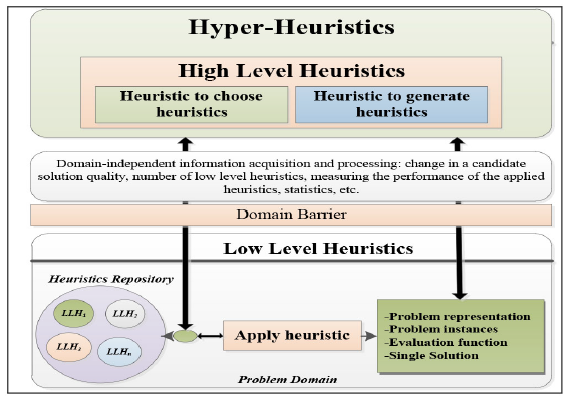
\includegraphics[scale=0.6]{figures/hyperheuristic.png}
	\caption{General scheme of hyper-heuristic framework}
\end{figure}	



Recently Burke et al \cite{burke2010classification} classified hyper-heuristic frameworks based on the source of feedback during the learning process and the nature of the search space. In the case of the source of feedback Burke el al \cite{burke2010classification} mention 3 possibilities: online, offline and no learning. If the hyper-heuristic framework uses information gathered during the problem solving it is considered as an online framework. An offline framework requires a training phase to gather information in order to use later in the validation phase. No learning occurs when no feedback is provided to the hyper-heuristic framework \cite{sabar2015automatic}. The nature of the search space can be either selecting or generating heuristics for the underlying problem. Next will be analyzed both kinds of high-level heuristics.

\begin{itemize}
	\item Selecting Heuristics: The majority of hyper-heuristic frameworks published define high level heuristics to select low level heuristics. In general, these frameworks operate using a set of human-designed low level heuristics, usually called pool of heuristics. The pool can contain both constructive or perturbative heuristics. The objective of the hyper-heuristic framework is to select the heuristic, from the pool, which most suits at a given moment. The main idea behind this: is that the strength of several heuristics can be combined into a single framework in order to better explore the search space. Most of the proposed selection mechanisms use simple rules to select the low level heuristics based on their past performance \cite{sabar2015automatic}.
	\item Generating Heuristics: In this case, the hyper-heuristic framework starts with a set subcomponents from low level heuristics and have the goal of fabricate new low level heuristics with it. Genetic programming is reported as a good strategy to combine and generated new heuristics for the SAT, scheduling and bin-packing problems \cite{sabar2015automatic}.
\end{itemize}



\section{Genetic Programming}

Genetic Programming (GP) \cite{burke2009exploring} is a sub-field from the program synthesis which uses ideas from the evolution theory to produce programs. The principle factors from the evolutionary computation are inheritance, reproduction/mutation and selection of the fittest. These factors drives the evolution of programs using genetic programming. Initially, a random-generated population of programs is created. Using a selection method to select good individuals for reproduction. Then the reproduction and mutation steps takes place in order to generate an offspring. Finally, the offspring is evaluated to assign a fitness value and based on this value the offspring can either enter or not in the population. Genetic programming is a method to generate syntactically valid programs and the fitness function is used to decide which one is the most suitable for a given problem. Traditionally in genetic programming, the programs that compose the population are represented using a tree structure. However, other structures that can be evolved exists, for instance: linear sequences of instructions and grammatic expressions. 

\section{Grammatical Evolution} 

Grammatical Evolution (GE) is a relatively new technique from the evolutionary computing, introduced by Ryan el al. \cite{ryan1998grammatical} and it is a type of GP which utilizes a grammatic to generate programs. Just like in GP the main goal is to find a executable program or piece of code, which have a good fitness value. Ryan el al. \cite{ryan1998grammatical} proposes one technique to generate programs or fragments for any language using BNF definitions. This technique can be used to evolve programs though a evolution process. The GE uses a mapping mechanism between the genotype (coded individuals by integer vectors) and phenotype (generated programs to resolve a problem). The Backus Naur Form (BNF) notation is used to represent a grammatic from a language in form of production rules. A BNF grammatic consists in a set of terminals, which are items that are allowed to the language, for instance: +, -, *, / etc and non-terminals, which can be expanded into one or more terminals. The grammatic can be expressed as a tuple ${N,T,P,S}$, where $N$ is a set of non-terminals, $T$ a set of terminals, $P$ a set of production rules that maps the elements $N$ to $T$; finally, $S$, a symbol to represent the initial point contained in $N$.
 
\begin{center}
	
	$ N = {\langle expr \rangle, \langle op \rangle, \langle pre-op \rangle}$
	
	$ T = {Sin,Cos,Tan,Log,+,-,/,*,X} $
	
	$ S = \langle expr \rangle $
	
\end{center}

\noindent
E $P$ pode ser representada como:

\begin{Grammar}
	\begin{grammar}
		
		
		<expr> ::=  <expr> <op> <expr> \hspace{2cm} (0) 
		\alt (<expr> <op> <expr>)  \hspace{1.75cm}  (1)  
		\alt <pre-op> (<expr>) \hspace{2.2cm}  (2) \alt <var> \hspace{3.9cm} (3) \\\
		
		<op> ::=  + \hspace{4.4cm} (0)   \alt - \hspace{4.5cm}  (1)  \alt  /  \hspace{4.51cm}  (2) \alt * \hspace{4.45cm}  (3) \\
		
		<pre-op> ::= Sin \hspace{4.2cm} (0) \alt Cos
	\hspace{4.12cm} (1) \alt Tan  \hspace{4.13cm} (2) \alt Cos \hspace{4.12cm} (3) \\
		
		<var> ::= X  \hspace{4.4cm} (0)
		
		
	\end{grammar}
	
	\caption{Gramática exemplo para demonstrar como decodificar vetores de inteiros em programas de computador.}
	\label{gram:gramatica}
\end{Grammar}


\begin{table}[htb]
	\centering
	\caption{\textit{Regras de produção} e o número de escolhas para cada uma.}
	\label{tab:productionRules}
	\begin{tabular}{|l|l|}
		\hline
		Production Rules & Number of choices \\ \hline
		$\langle expr \rangle$                        & 4       \\ \hline
		$\langle op \rangle$                         & 4       \\ \hline
		$\langle pre-op \rangle$                         & 4       \\ \hline
		$\langle var \rangle$                          & 1       \\ \hline
	\end{tabular}
\end{table}


Ryan et al. \cite{ryan1998grammatical}  proposed the use of genetic algorithm (GA) to control which choices should be made, in this sense allowing the GA select which production rules should be utilized. An individual (chromosome) consists in variable-length vector of integers and it is called the genotype. 

% Para fins de compreensão o processo de mapeamento de um cromossomo será demonstrado utilizando a \autoref{gram:gramatica} apresentada anteriormente nesta seção. O Algoritmo \ref{alg:pseudocodigogrammar} apresenta o \textit{template} geral dos programas gerados pela \autoref{gram:gramatica}. A expressão $\langle expr \rangle$ apresentada na linha 2 do Algoritmo \ref{alg:pseudocodigogrammar} é substituída por expressões matemáticas que estão codificadas pelos cromossomos (vetores de inteiros). 





\subsubsection{Subsubsection Heading Here}
Subsubsection text here.


% An example of a floating figure using the graphicx package.
% Note that \label must occur AFTER (or within) \caption.
% For figures, \caption should occur after the \includegraphics.
% Note that IEEEtran v1.7 and later has special internal code that
% is designed to preserve the operation of \label within \caption
% even when the captionsoff option is in effect. However, because
% of issues like this, it may be the safest practice to put all your
% \label just after \caption rather than within \caption{}.
%
% Reminder: the "draftcls" or "draftclsnofoot", not "draft", class
% option should be used if it is desired that the figures are to be
% displayed while in draft mode.
%
%\begin{figure}[!t]
%\centering
%\includegraphics[width=2.5in]{myfigure}
% where an .eps filename suffix will be assumed under latex, 
% and a .pdf suffix will be assumed for pdflatex; or what has been declared
% via \DeclareGraphicsExtensions.
%\caption{Simulation results for the network.}
%\label{fig_sim}
%\end{figure}

% Note that the IEEE typically puts floats only at the top, even when this
% results in a large percentage of a column being occupied by floats.


% An example of a double column floating figure using two subfigures.
% (The subfig.sty package must be loaded for this to work.)
% The subfigure \label commands are set within each subfloat command,
% and the \label for the overall figure must come after \caption.
% \hfil is used as a separator to get equal spacing.
% Watch out that the combined width of all the subfigures on a 
% line do not exceed the text width or a line break will occur.
%
%\begin{figure*}[!t]
%\centering
%\subfloat[Case I]{\includegraphics[width=2.5in]{box}%
%\label{fig_first_case}}
%\hfil
%\subfloat[Case II]{\includegraphics[width=2.5in]{box}%
%\label{fig_second_case}}
%\caption{Simulation results for the network.}
%\label{fig_sim}
%\end{figure*}
%
% Note that often IEEE papers with subfigures do not employ subfigure
% captions (using the optional argument to \subfloat[]), but instead will
% reference/describe all of them (a), (b), etc., within the main caption.
% Be aware that for subfig.sty to generate the (a), (b), etc., subfigure
% labels, the optional argument to \subfloat must be present. If a
% subcaption is not desired, just leave its contents blank,
% e.g., \subfloat[].


% An example of a floating table. Note that, for IEEE style tables, the
% \caption command should come BEFORE the table and, given that table
% captions serve much like titles, are usually capitalized except for words
% such as a, an, and, as, at, but, by, for, in, nor, of, on, or, the, to
% and up, which are usually not capitalized unless they are the first or
% last word of the caption. Table text will default to \footnotesize as
% the IEEE normally uses this smaller font for tables.
% The \label must come after \caption as always.
%
%\begin{table}[!t]
%% increase table row spacing, adjust to taste
%\renewcommand{\arraystretch}{1.3}
% if using array.sty, it might be a good idea to tweak the value of
% \extrarowheight as needed to properly center the text within the cells
%\caption{An Example of a Table}
%\label{table_example}
%\centering
%% Some packages, such as MDW tools, offer better commands for making tables
%% than the plain LaTeX2e tabular which is used here.
%\begin{tabular}{|c||c|}
%\hline
%One & Two\\
%\hline
%Three & Four\\
%\hline
%\end{tabular}
%\end{table}


% Note that the IEEE does not put floats in the very first column
% - or typically anywhere on the first page for that matter. Also,
% in-text middle ("here") positioning is typically not used, but it
% is allowed and encouraged for Computer Society conferences (but
% not Computer Society journals). Most IEEE journals/conferences use
% top floats exclusively. 
% Note that, LaTeX2e, unlike IEEE journals/conferences, places
% footnotes above bottom floats. This can be corrected via the
% \fnbelowfloat command of the stfloats package.




\section{Conclusion}
The conclusion goes here.




% conference papers do not normally have an appendix


% use section* for acknowledgment
\section*{Acknowledgment}


The authors would like to thank...





% trigger a \newpage just before the given reference
% number - used to balance the columns on the last page
% adjust value as needed - may need to be readjusted if
% the document is modified later
%\IEEEtriggeratref{8}
% The "triggered" command can be changed if desired:
%\IEEEtriggercmd{\enlargethispage{-5in}}

% references section

% can use a bibliography generated by BibTeX as a .bbl file
% BibTeX documentation can be easily obtained at:
% http://mirror.ctan.org/biblio/bibtex/contrib/doc/
% The IEEEtran BibTeX style support page is at:
% http://www.michaelshell.org/tex/ieeetran/bibtex/
%\bibliographystyle{IEEEtran}
% argument is your BibTeX string definitions and bibliography database(s)
%\bibliography{IEEEabrv,../bib/paper}
%
% <OR> manually copy in the resultant .bbl file
% set second argument of \begin to the number of references
% (used to reserve space for the reference number labels box)
	%Referências
	\bibliographystyle{plain}
	\bibliography{references}



% that's all folks
\end{document}


